Um die oben genannten Spiele um einen virtuellen Teil erweitern zu können werden Konzepte benötigt. Eine von uns getroffene Auswahl wird im folgenden beschrieben. 

\section{Erweiterte Realität}
Konzepte, die explizit die Realität erweitern und somit einen Mehrwert zum Spiel beitragen.


\subsubsection{Integration virtueller Objekte in die physische Umgebung}
Um ein virtuelles Spiel in die physische Umgebung integrieren zu können, müssen auch alle Objekte
des virtuelles Spieles in die physische Umgebung gebracht werden.
Bei vielen Objekten kann dies durch einen eingeschränkten Zufall geschehen. Z.B. bei Snake die 
Items. Bei dem ein oder anderen Spiel soll es eine Basis für jedes Team geben. Dabei bietet sich an
dieses auf eine relativ freie Fläche festzusetzen. Generell sollte darauf geachtet werden, 
dass die Objekte nicht innerhalb eines Gebäudes landen oder in nicht begehbares Terrain platziert werden.



Dies kann mit Hilfe der folgenden technischen Lösungen umgesetzt werden:
Kartendarstellung (s. \ref{kartendarstellung}), Kollisionsabfrage (s. \ref{kollisionsabfrage}), Positionsabfrage (um sicherzustellen, dass das Objekt in der Nähe des Spieler erstellt wird, s. \ref{positionsermittlung}).

\subsubsection{Darstellung der physischen und virtuellen Umgebung}

Die physische Welt in eine virtuelle Umgebung zu übertragen kann oft sehr hilfreich sein.
Sei es in einer Karte als Übersicht oder lediglich eine Anzeige ob man sich innerhalb bzw.
außerhalb des Spielfelds befindet. 
\begin{figure}[htbp]
  \centering
    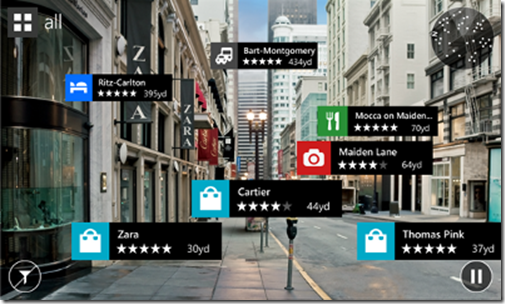
\includegraphics[width=0.9\textwidth]{3-Spielkonzepte/3-1-Erweiterte_Realitaet/map01.png}
     \caption{Handyscreen um die zu sehenden Geschäfte, Hotels, etc. erweitert
	(Quelle: \url{http://blogs.bing.com/maps/wp-content/uploads/sites/3/2013/06/clip_5F00_image006_5F00_thumb_5F00_4AEFDB0C.png})
		}
\end{figure}
Eine Karte hat insoweit den Vorteil, dass man dort auch
virtuelle Gegenstände einfügen kann, die in der physischen Welt nicht vorhanden
sind, wie beispielsweise die nächsten Items bei Snake.
Dazu sind 
Kartendarstellung (s. \ref{kartendarstellung}) und Positionsermittlung (s. \ref{positionsermittlung}) nötig.

\subsubsection{Kollision virtueller Objekte}
Treffen zwei virtuelle Objekte aufeinander muss in der Regel ein Event ausgelöst werden.
Wird bei Snake z.B. der eigene Schwanz berührt, was laut der Regeln nicht erlaubt ist, muss
dies dem Spieler mitgeteilt werden und evtl. weitere Ereignisse ausgeführt werden.
\newline
Technische Lösungen:
Kollisionsabfrage (s. \ref{kollisionsabfrage}), Positionsermittlung (s. \ref{positionsermittlung})


\subsubsection{Einsammeln von Objekten}
Eine Variante der Kollision mit virtuellen Objekten ist das Einsammeln. Wenn ein Spieler in
Reichweite eines Items ist, das es einzusammeln gilt, kann dies entweder automatisch
passieren oder über eine Aufforderung auf dem mobilen Gerät. Zur Bestätigung, dass
etwas eingesammelt wurde, kann nun wiederum ein akustisches oder haptisches Signal
gegeben werden.


Technische Lösungen:
Positionsermittlung (s. \ref{positionsermittlung}), Kollisionsabfrage (s. \ref{kollisionsabfrage})
